In this section, we evaluate the performance of the proposed framework. Our
prototype of the framework is implemented in the Go programming language, and
the corresponding source code is available online \cite{sources}. The framework
is divided into multiple libraries, each of which can be used independently. The
source code of the experimental setup below along with the input data are also
available at \cite{sources}. The experiments are conducted on a GNU/Linux
machine equipped with 16 processors Intel Xeon E5520 2.27~GHz and 24~GB of RAM.

Each problem that we consider is structured as follow. A platform $\procs$ with
$\np$ processing elements and an application $\tasks$ with $\nt$ tasks are
generated randomly by the \abbr{TGFF} tool \cite{dick1998}. The tool generates
$\np$ tables and a directed acyclic graph with $\nt$ nodes. Each table
corresponds to a processing element, and it describes certain properties of the
tasks when they are mapped to that particular processing element. Namely, each
table assigns two numbers to each task: a reference execution time, chosen
uniformly between 10 and 50~ms, and a power consumption, chosen uniformly
between 5 and 15~W. The graph captures data dependencies between the tasks. The
application is scheduled using a list scheduler \cite{adam1974}. The mapping of
the application is fixed and obtained by scheduling the tasks based on their
reference execution times and assigning them to the earliest available
processing elements (a shared ready list).

The construction of thermal \abbr{RC} circuits needed for temperature analysis
is delegated to the HotSpot tool \cite{skadron2004}. The floorplan of each
platform is a regular grid wherein each processing element occupies $2 \times
2~\text{mm}^2$ on the die. The output of the tool is essentially a pair of a
thermal capacitance matrix $\mC$ and a thermal conductance $\mG$ matrix needed
in \eref{thermal-system}. The leakage modeling is based on a linear
approximation \cite{yang2013, ukhov2012, liu2007}.

\begin{figure}[t]
  \centering
  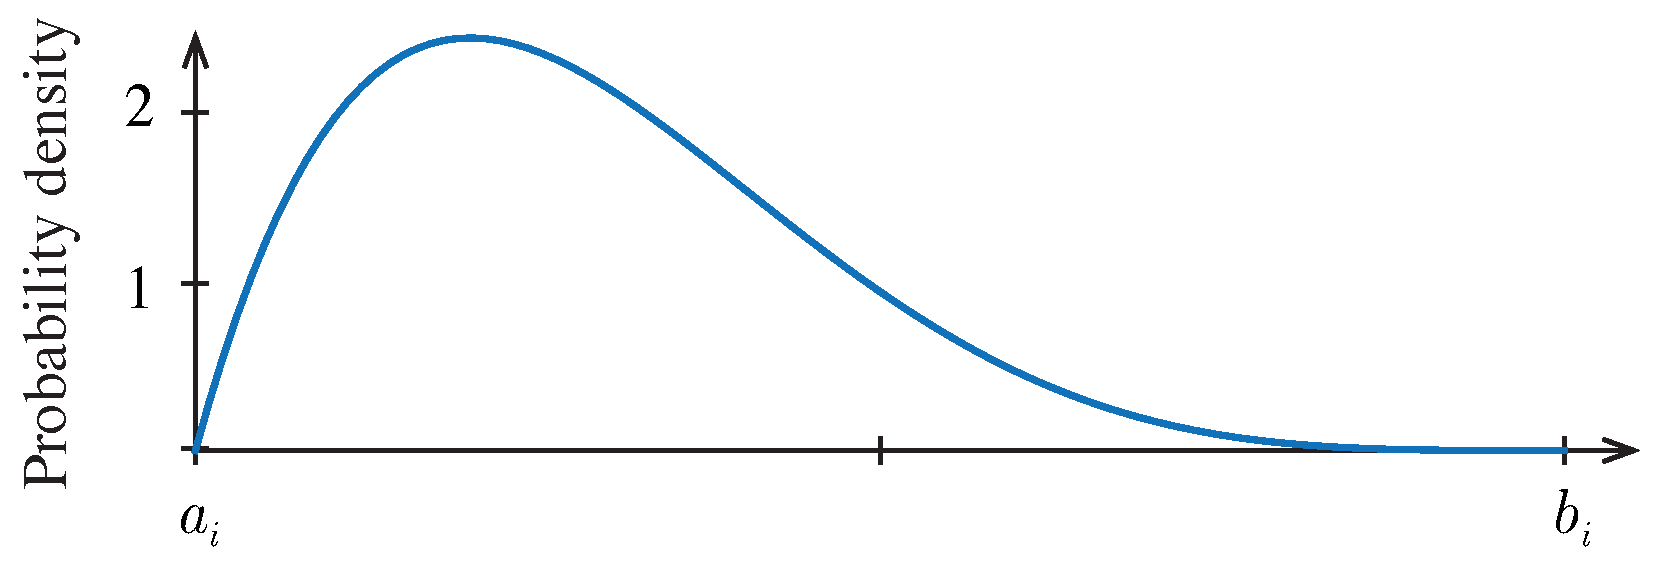
\includegraphics[width=1.0\columnwidth]{include/assets/figures/beta.pdf}
  \caption{The probability density of the beta distribution $\text{Beta}(2, 5, a_i, b_i)$.}
  \flab{beta}
\end{figure}

The uncertain parameters $\vu$ are the execution times of the tasks; all other
parameters are deterministic. Targeting the practical scenario described in
\sref{uncertain-parameters}, the marginal distributions and correlation matrix
of $\vu$ are assumed to be available. Without loss of generality, the marginal
of $\u_i$ is a four-parametric beta distribution $\text{Beta}(\alpha_i, \beta_i,
a_i, b_i)$ where $\alpha_i$ and $\beta_i$ are the shape parameters, and $a_i$
and $b_i$ are the endpoints of the support. The left endpoint $a_i$ is set to
the reference execution time generated by the \abbr{TGFF} tool as discussed
earlier, and the right endpoint $b_i$ is set to be 20\% larger than $a_i$. The
parameters $\alpha_i$ and $\beta_i$ are set to two and five, respectively, for
all tasks, skewing their uncertain execution times towards the reference
execution times. The probability density function of such a distribution is
depicted in \fref{beta}. The correlations between the tasks are computed based
on the structure of the graph produced by the \abbr{TGFF} tool: the closer two
tasks are in the graph, the stronger their execution times are correlated.

The quantities of interest $\g$ that we shall consider are the end-to-end delay
of the application, the total energy consumed by the processing elements, and a
temperature profile of the system given by \eref{end-to-end-delay},
\eref{total-energy}, and \eref{temperature-profile}, respectively.

Regarding the interpolation algorithm, we rely on the open Newton--Cotes rule as
motivated in \sref{collocation-nodes}. The \token{IsEnough} subroutine of
\aref{construct} terminates the algorithm when it reaches a certain
interpolation level. The decision taken in \token{IsAccurate} is based on the
formula given in \eref{error}.

Lastly, we would like to remind that our setup is publicly available
\cite{sources}. The configuration aspects that have not been explicitly
mentioned here can be found online, and the results presented below can be
readily reproduced.

\subsection{End-to-End Delay}
\begin{table*}
  \caption{End-to-end delay}
  \begin{tabular*}{\textwidth}{=R{10pt}-R{25pt}-R{50pt}-R{25pt}-R{50pt}-R{25pt}-R{50pt}-R{25pt}-R{50pt}-R{25pt}-R{50pt}}
    \toprule
    & \multicolumn{2}{c}{2/20} & \multicolumn{2}{c}{4/40} & \multicolumn{2}{c}{8/80} & \multicolumn{2}{c}{16/160} & \multicolumn{2}{c}{32/320} \\
    \cmidrule( r){1-1}
    \cmidrule(l ){2-3}
    \cmidrule(l ){4-5}
    \cmidrule(l ){6-7}
    \cmidrule(l ){8-9}
    \cmidrule(l ){10-11}
     2 &  31 & $2.69 \times 10^{-2}$ &  67 & $2.64 \times 10^{-2}$ & 119 & $2.83 \times 10^{-2}$ & 187 & $2.82 \times 10^{-2}$ &  965 & $2.62 \times 10^{-2}$ \\
     4 &  67 & $1.12 \times 10^{-2}$ & 176 & $1.05 \times 10^{-2}$ & 245 & $1.24 \times 10^{-2}$ & 531 & $1.78 \times 10^{-2}$ & 2207 & $1.37 \times 10^{-2}$ \\
     6 &  85 & $5.88 \times 10^{-3}$ & 236 & $5.85 \times 10^{-3}$ & 315 & $7.56 \times 10^{-3}$ & 692 & $1.29 \times 10^{-2}$ & 2795 & $1.02 \times 10^{-2}$ \\
     8 &  97 & $4.29 \times 10^{-3}$ & 256 & $5.26 \times 10^{-3}$ & 343 & $6.84 \times 10^{-3}$ & 728 & $1.28 \times 10^{-2}$ & 3089 & $9.48 \times 10^{-3}$ \\
    10 & 109 & $3.84 \times 10^{-3}$ & 276 & $5.22 \times 10^{-3}$ & 371 & $6.78 \times 10^{-3}$ & 764 & $1.28 \times 10^{-2}$ & 3257 & $9.34 \times 10^{-3}$ \\
    \bottomrule
  \end{tabular*}
  \tlab{end-to-end-delay}
\end{table*}
% vim: nowrap tw=0

The quantity of interest $\g$ considered in this subsection is the end-to-end
delay given in \eref{end-to-end-delay}, which is a scalar.

\subsection{Total Energy}
\begin{table*}
  \caption{Total energy}
  \begin{tabular*}{\textwidth}{=R{10pt}-R{25pt}-L{50pt}-R{25pt}-L{50pt}-R{25pt}-L{50pt}-R{25pt}-L{50pt}-R{25pt}-L{50pt}}
    \toprule
    & \multicolumn{2}{c}{1/10} & \multicolumn{2}{c}{4/40} & \multicolumn{2}{c}{9/90} & \multicolumn{2}{c}{16/160} & \multicolumn{2}{c}{25/250} \\
    \cmidrule( r){1-1}
    \cmidrule(l ){2-3}
    \cmidrule(l ){4-5}
    \cmidrule(l ){6-7}
    \cmidrule(l ){8-9}
    \cmidrule(l ){10-11}
     2 & 0 & $0.00 \times 10^{-0}$ & 0 & $0.00 \times 10^{-0}$ & 0 & $0.00 \times 10^{-0}$ & 0 & $0.00 \times 10^{-0}$ & 0 & $0.00 \times 10^{-0}$ \\
     4 & 0 & $0.00 \times 10^{-0}$ & 0 & $0.00 \times 10^{-0}$ & 0 & $0.00 \times 10^{-0}$ & 0 & $0.00 \times 10^{-0}$ & 0 & $0.00 \times 10^{-0}$ \\
     6 & 0 & $0.00 \times 10^{-0}$ & 0 & $0.00 \times 10^{-0}$ & 0 & $0.00 \times 10^{-0}$ & 0 & $0.00 \times 10^{-0}$ & 0 & $0.00 \times 10^{-0}$ \\
     8 & 0 & $0.00 \times 10^{-0}$ & 0 & $0.00 \times 10^{-0}$ & 0 & $0.00 \times 10^{-0}$ & 0 & $0.00 \times 10^{-0}$ & 0 & $0.00 \times 10^{-0}$ \\
    10 & 0 & $0.00 \times 10^{-0}$ & 0 & $0.00 \times 10^{-0}$ & 0 & $0.00 \times 10^{-0}$ & 0 & $0.00 \times 10^{-0}$ & 0 & $0.00 \times 10^{-0}$ \\
    \bottomrule
  \end{tabular*}
  \tlab{total-energy}
\end{table*}
% vim: nowrap tw=0

Let the quantity of interest $\g$ be the total energy given in
\eref{total-energy}, which is a scalar.

\subsection{Temperature Profile}
\begin{table*}
  \caption{Temperature profile}
  \begin{tabular*}{\textwidth}{=R{10pt}-R{25pt}-R{50pt}-R{25pt}-R{50pt}-R{25pt}-R{50pt}-R{25pt}-R{50pt}-R{25pt}-R{50pt}}
    \toprule
    & \multicolumn{2}{c}{2/20} & \multicolumn{2}{c}{4/40} & \multicolumn{2}{c}{8/80} & \multicolumn{2}{c}{16/160} & \multicolumn{2}{c}{32/320} \\
    \cmidrule( r){1-1}
    \cmidrule(l ){2-3}
    \cmidrule(l ){4-5}
    \cmidrule(l ){6-7}
    \cmidrule(l ){8-9}
    \cmidrule(l ){10-11}
     2 & 0 & $0.00 \times 10^{-0}$ & 0 & $0.00 \times 10^{-0}$ & 0 & $0.00 \times 10^{-0}$ & 0 & $0.00 \times 10^{-0}$ & 0 & $0.00 \times 10^{-0}$ \\
     4 & 0 & $0.00 \times 10^{-0}$ & 0 & $0.00 \times 10^{-0}$ & 0 & $0.00 \times 10^{-0}$ & 0 & $0.00 \times 10^{-0}$ & 0 & $0.00 \times 10^{-0}$ \\
     6 & 0 & $0.00 \times 10^{-0}$ & 0 & $0.00 \times 10^{-0}$ & 0 & $0.00 \times 10^{-0}$ & 0 & $0.00 \times 10^{-0}$ & 0 & $0.00 \times 10^{-0}$ \\
     8 & 0 & $0.00 \times 10^{-0}$ & 0 & $0.00 \times 10^{-0}$ & 0 & $0.00 \times 10^{-0}$ & 0 & $0.00 \times 10^{-0}$ & 0 & $0.00 \times 10^{-0}$ \\
    10 & 0 & $0.00 \times 10^{-0}$ & 0 & $0.00 \times 10^{-0}$ & 0 & $0.00 \times 10^{-0}$ & 0 & $0.00 \times 10^{-0}$ & 0 & $0.00 \times 10^{-0}$ \\
    \bottomrule
  \end{tabular*}
  \tlab{temperature-profile}
\end{table*}
% vim: nowrap tw=0

In this subsection, the quantity of interest $\g$ is the temperature profile
$\mQ$ of the system calculated using \eref{thermal-system}. The profile is an
$\np \times \ns$ matrix, and, therefore, $\g$ is $\np \ns$-dimensional.
